\documentclass[a4paper,11.5pt]{article}
\usepackage[textwidth=170mm, textheight=230mm, inner=20mm, top=20mm, bottom=30mm]{geometry}
\usepackage[normalem]{ulem}
\usepackage[utf8]{inputenc}
\usepackage[T1]{fontenc}
\PassOptionsToPackage{defaults=hu-min}{magyar.ldf}
\usepackage[magyar]{babel}
\usepackage{amsmath, xcolor, amsthm,amssymb,paralist,array, ellipsis, graphicx, tikz}
\usetikzlibrary{shapes.geometric, arrows, positioning}
%\usepackage{marvosym}

\usepackage{listings}
\lstset{
	language=C++, 
	basicstyle=\ttfamily, 
	keywordstyle=\color{blue}\ttfamily, 
	stringstyle=\color{red}\ttfamily,
	tabsize = 4
}

\makeatletter
\renewcommand*{\mathellipsis}{%
	\mathinner{%
		\kern\ellipsisbeforegap%
		{\ldotp}\kern\ellipsisgap%
		{\ldotp}\kern\ellipsisgap%
		{\ldotp}\kern\ellipsisaftergap%
	}%
}
\renewcommand*{\dotsb@}{%
	\mathinner{%
		\kern\ellipsisbeforegap%
		{\cdotp}\kern\ellipsisgap%
		{\cdotp}\kern\ellipsisgap%
		{\cdotp}\kern\ellipsisaftergap%
	}%
}
\renewcommand*{\@cdots}{%
	\mathinner{%
		\kern\ellipsisbeforegap%
		{\cdotp}\kern\ellipsisgap%
		{\cdotp}\kern\ellipsisgap%
		{\cdotp}\kern\ellipsisaftergap%
	}%
}
\renewcommand*{\ellipsis@default}{%
	\ellipsis@before
	\kern\ellipsisbeforegap
	.\kern\ellipsisgap
	.\kern\ellipsisgap
	.\kern\ellipsisgap
	\ellipsis@after\relax}
\renewcommand*{\ellipsis@centered}{%
	\ellipsis@before
	\kern\ellipsisbeforegap
	.\kern\ellipsisgap
	.\kern\ellipsisgap
	.\kern\ellipsisaftergap
	\ellipsis@after\relax}
\AtBeginDocument{%
	\DeclareRobustCommand*{\dots}{%
		\ifmmode\@xp\mdots@\else\@xp\textellipsis\fi}}
\def\ellipsisgap{.1em}
\def\ellipsisbeforegap{.05em}
\def\ellipsisaftergap{.05em}
\makeatother

\usepackage{hyperref}

\begin{document}
	%%%%%%%%%%%RÖVIDÍTÉSEK%%%%%%%%%%
	\setlength\parindent{0pt}
	\def\s{\hspace{0.2mm}\vphantom{\beta}}
	\def\Z{\mathbb{Z}}
	\def\Q{\mathbb{Q}}
	\def\R{\mathbb{R}}
	\def\C{\mathbb{C}}
	\def\N{\mathbb{N}}
	\def\Ra{\overline{\mathbb{R}}}
	
	\def\sume{\displaystyle\sum_{n=1}^{+\infty}}
	\def\sumn{\displaystyle\sum_{n=0}^{+\infty}}
	
	\def\narrow{\underset{n\rightarrow+\infty}{\longrightarrow}}
	\def\limn{\displaystyle\lim_{n\to +\infty}}
	\def\limx{\displaystyle\lim_{x\to +\infty}}
	
	\theoremstyle{definition}
	\newtheorem{theorem}{Tétel}[subsection] 
	
	\theoremstyle{definition}
	\newtheorem{definition}[theorem]{Definíció} 
	\newtheorem{example}[theorem]{Példa} 
	\newtheorem{task}[theorem]{Feladat} 
	\newtheorem{note}[theorem]{Megjegyzés}
	%%%%%%%%%%%%%%%%%%%%%%%%%%%%%%%%%%%%%%%%%%%%%%%%%%%%%%%%%%%%%%%%%%%%%
	\begin{center}
		{\LARGE\textbf{C++}}
		
		{\Large Gyakorlat jegyzet}
		
		1. óra
	\end{center}
	A jegyzetet \textsc{Umann} Kristóf készítette \textsc{Horváth} Gábor gyakorlatán. (\today)
	\section{Bevezető}
	A C++ többek között a hatákonyságáról is híres. Andrei Alexandrescu azt nyilatkozta, hogy amikor a Facebooknál a backend kódján 1\%ot sikerült optimalizálni, több mint 10 évnyi fizetését spórolta meg a cégnek havonta csak az áramköltségen. Nem használ garbage collectort: nincs nem várt szünet a program végrehajtásában a menedzselt nyelvekkel szemben.

  A C++-szal kapcsolatban az egyik gyakori tévhoz, hogy egy alacsony szintű nyelvről van szó. Bár a nyelv lehetőséget biztosít arra, hogy alacsony szinten hozzáférjünk a hardvereinkhez, számos gazdag absztrakciós lehetőséget tartalmaz. Ezeknek a használatával magas szintű kód írására is kíválóan alkalmas. A legtöbb nyelvhez képest abban emelkedik ki, hogy a C++ nyelvben ezeknek az absztrakcióknak ritkán van futási idejű költsége. Legtöbbször a fordítóprogram teljesen el tudja tüntetni ezeket az absztrakciókat a programból a fordítás során.

  A C++ filozófiájának fontos eleme, hogy ha nem használunk egy adott nyelvi eszközt, akkor annak ne legyen hatása a program teljesítményére.

  Fontos, hogy a C++ alapvetően nem egy objektum orientált nyelv. Bár számos nyelvi eszköz támogatja az objektum orientált stílusú programozást, de a nyelv kíválóan alkalmas más paradigmák használatára is. A funkcionális programozástól a generatív programozáson át a deklaratív stílusig sok programozási stílusra alkalmas. A nyelv nem próbál ráerőltetni egy megközelítést a programozóra, ellenben próbál minél gazdagabb eszköztárat biztosítani, hogy a megfelelő problémát a lehető legmegfelelőbb módon lehessen megoldani. Még akkor is, ha ez a különböző paradigmák keverését vonja maga után. Ezért ezt a nyelvet gyakran multiparadigmás programozási nyelvnek szokták hívni. 
	
	\medskip
	Cél: a tárgy során kialakítani a nyelvvel kapcsolatban egy intuíciót, ami segítéségével elkerülhetőek alapvető hibák is. Az előzménytárgyakban az egyszerűség kedvéért gyakran féligazságok hangzottak el, ezeket is helyre kell rakni.
	\subsection{Mi az a C++?}
  Alapvetően a nyelv két összetevőből áll. Az aktuális szabványból és annak implementációiból (fordítók + szabványkönyvtárak). A szabvány, ami meghatározza a nyelv nyelvtanját, valamint a szemantikát: mit jelentenek a leforduló programok (nem definiál minden részletet). Emellett a szabvány definiálja a szabványkönyvtárat is, amit minden szabványos C++ fordító mellé szállítani kell. Az első C++ szabvány a {C++98} volt. További szabványai: {C++03}, {C++11}, {C++14}, {C++17}.
	
	\medskip
  %% TODO linkek.
  A szabvány alapján számos fordító (implementáció) létezik a C++ kódok fordítására: MSVC (Visual Studio), GCC, Clang.
  Létezik számos fejlesztői környezet is, mint például: CLion, QtCreator, CodeBlocks, VIM. De ezek nem fordítók, legtöbbször a fent említett fordítók közül használnak egyet.
  \section{Különböző viselkedések kategorizálása} 

  Egy reménytelen megközelítés lenne a szabványban minden szintaktikusan (nyelvtanilag) helyes kódhoz pontos szemantikát (működést) társítani. Ennek mind elméleti és gyakorlati oka van. Ezért a C++ szabvány néhány esetben nem vagy csak részben definiálja egy adott program működését. A következőkben erre fogunk példákat látni.

	\subsection{Nem definiált viselkedések}
	\begin{lstlisting}
int main()
{
	int i = 0;
	std::cout << i++ << i++ << std::endl;
}
	\end{lstlisting}
  Lehetséges kimenet: \texttt{01} (GCC 6.1 fordítóval 64 bites x86 Linux platformon)
	
	Lehetséges kimenet: \texttt{10} (Clang 3.9 fordítóval 64 bites x86 Linux platformon)
	\medskip
	
	Fordítás és futtatás után különböző eredményeket kaphatunk, mert itt az, hogy mikor értékelődik ki a két \texttt{++i} a kifejezésen belül, az \textbf{nem specifikált.} Ha a szabvány nem terjed ki arra, hogy milyen viselkedésű kódot generáljon a fordító, akkor a fordító bármit választhat. 
	\medskip
	
	Gyakran eldönthetetlen előre, hogy mikor mi lesz a leghatékonyabb megoldás, ez az egyik ok, hogy nem definiál mindent a szabvány.
	\medskip
	
	Ez lehetőséget ad a fordítónak arra, hogy \textbf{optimalizáljon.} 
	\medskip
	
	A C++ban van un. szekvenciapontok, és a szabvány csak azt mondja ki, hogy a szekvenciapont előtti kód hamarabb kerüljön végrehajtásra mint az utána levő. Mivel itt az \textit{i} értékadása után és csak az \texttt{std::endl} után van szekvenciapont, így az, hogy milyen sorrendben történjen a kettő közötti kifejezés részkifejezéseinek a kiértékelése, az a fordítóra van bízva.
	\medskip
	
	A C++ban nem meghatározott, hogy két szekvenciapont között mi az utasítások végrehajtásának a sorrendje.
	
	\medskip
	Az, hogy két részkifejezés szekvenciaponttal történő elválasztás nélkül ugyanazt a memóriaterületet módosítja, \textbf{nem definiált} viselkedést eredményez. Nem definiált viselkedés esetén a fordító vagy a futó program bármit csinálhat. A szabvány semmiféle megkötést nem tesz.
	\begin{note}
		Az a program, amely nem definiált viselkedéseket tartalmaz, hibás.
	\end{note}
	\subsection{Nem specifikált viselkedések}
	Amennyiben a szabvány definiál néhány lehetséges opciót, de a fordítóra bízza, hogy az melyiket választja, akkor \textbf{nem specifikált} viselkedésről beszélünk.
	
  A nem specifikált viselkedés csak akkor probléma, ha a program végeredményét (megfigyelhető működését) befolyásolhatja a fordító választása. Például a fenti kódot módosíthatjuk a következő képpen:
	
	\begin{example}\ 
		
		\begin{lstlisting}
int main()
{
	int i = 0;
	int j = 0;
	std::cout << ++i << ++j << std::endl; // 11
}
		\end{lstlisting}
	\end{example}
	Bár azt továbbra se tudjuk, hogy \texttt{++i} vagy \texttt{++j} értékelődik ki hamarabb, (\textit{nem specifikált}), azt biztosan tudjuk, hogy 11-et fog kiírni (a program végeredménye \textit{jól definiált}).
	\subsection{Implementáció által definiált viselkedés}
	A szabvány nem köti meg, hogy egy \texttt{int} egy adott platformon mennyi byte-ból álljon. Ez állandó, egy adott platformon egy adott fordító mindig ugyanakkorát hoz létre, de platform/fordítóváltás esetén ez változhat. Ennek az az oka, hogy különböző platformokon különböző választás eredményez hatékony programokat. Ennek köszönhetően hatékony kódot tud generálni a fordító, viszont a fejlesztő dolga, hogy megbizonyosodjon róla, hogy az adott platformon a primitív típúsok méretei megfelelnek a program által elvárt követelményeknek.
	
	\section{A fordító működése}
	A fordítás 3 fő lépésből áll:
	\begin{compactenum}
		\item Preprocesszálás
		\item Fordítás (A tárgykód létrehozása)
		\item Linkelés (Szerkesztés)
	\end{compactenum}
	
	\begin{center}
		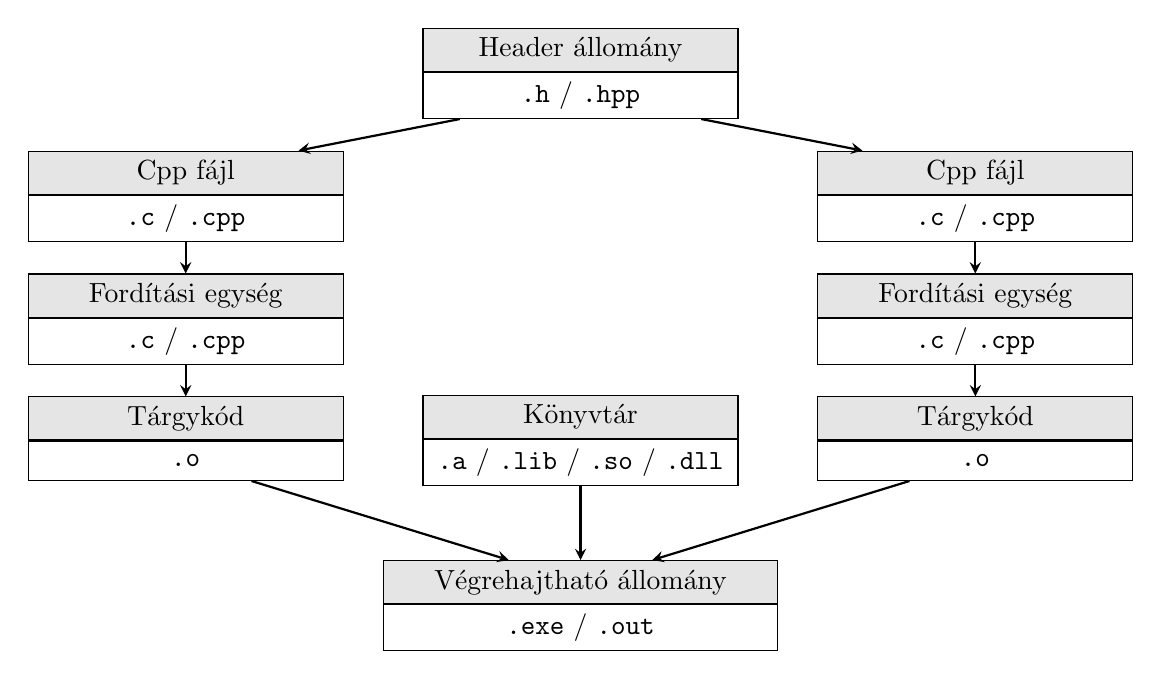
\begin{tikzpicture}
		\tikzstyle{Node} = [rectangle, minimum width=4cm, minimum height=5mm, text centered, draw=black, fill= gray!20]
		\tikzstyle{FileName} = [rectangle, minimum width=4cm, minimum height=5mm, text centered, draw=black, fill= white]
		\tikzstyle{NodeExe} = [rectangle, minimum width=5cm, minimum height=5mm, text centered, draw=black, fill= gray!20]
		\tikzstyle{FileNameExe} = [rectangle, minimum width=5cm, minimum height=5mm, text centered, draw=black, fill= white]
		\tikzstyle{arrow} = [thick,->,>=stealth]
		
		
		\node (header) [Node] {Header állomány};
		\node (headerFileName) [FileName, below = 0mm of header] {\texttt{.h} / \texttt{.hpp}};
		
		\node (cpp1) [Node, below left = of header] {Cpp fájl};
		\node (cpp1FileName) [FileName, below = 0mm of cpp1] {\texttt{.c} / \texttt{.cpp}};
		
		\node (cpp2) [Node, below right = of header] {Cpp fájl};
		\node (cpp2FileName) [FileName, below = 0mm of cpp2] {\texttt{.c} / \texttt{.cpp}};
		
		\node (translationUnit1) [Node, below = of cpp1] {Fordítási egység};
		\node (translationUnit1FileName) [FileName, below = 0mm of translationUnit1] {\texttt{.c} / \texttt{.cpp}};
		
		\node (translationUnit2) [Node, below = of cpp2] {Fordítási egység};
		\node (translationUnit2FileName) [FileName, below = 0mm of translationUnit2] {\texttt{.c} / \texttt{.cpp}};
		
		\node (objectFile1) [Node, below = of translationUnit1] {Tárgykód};
		\node (objectFile1FileName) [FileName, below = 0mm of objectFile1] {\texttt{.o}};
		
		\node (objectFile2) [Node, below = of translationUnit2] {Tárgykód};
		\node (objectFile2FileName) [FileName, below = 0mm of objectFile2] {\texttt{.o}};
		

		\node (libFile1) [Node, below = 4.1 cm of header] {Könyvtár};
		\node (libFile1FileName) [FileName, below = 0mm of libFile1] {\texttt{.a} / \texttt{.lib} / \texttt{.so} / \texttt{.dll}};
		
		\node (exe) [NodeExe, below = 6.2 cm of header] {Végrehajtható állomány};
		\node (exeFileName) [FileNameExe, below = 0mm of exe] {\texttt{.exe} / \texttt{.out}};
		
		
		\draw[arrow] (headerFileName) -- (cpp1);
		\draw[arrow] (headerFileName) -- (cpp2);
		\draw[arrow] (cpp1FileName) -- (translationUnit1);
		\draw[arrow] (cpp2FileName) -- (translationUnit2);
		\draw[arrow] (translationUnit1FileName) -- (objectFile1);
		\draw[arrow] (translationUnit2FileName) -- (objectFile2);
		\draw[arrow] (objectFile1FileName) -- (exe);
		\draw[arrow] (objectFile2FileName) -- (exe);
		\draw[arrow] (libFile1FileName) -- (exe);
		%TODO lehet az utolsó két oszlopot fel kéne cserélni
		
		\end{tikzpicture}
		\smallskip
		
		Szürkében az adott fordítási lépés neve, alatta az így létrehozott fájl kiterjesztése (leggyakrabban).	
	\end{center}
	A fordítás a preprocesszor parancsok végrehajtásával kezdődik (például a \textbf{header fájl}ok beillesztése a \textbf{cpp fájl}okba), az így kapott fájlot hívjuk \textbf{fordítási egység}nek (\textit{translation unit}). A fordítási egységek külön-külön fordulnak \textbf{tárgykód}dá (\textit{object file}). Ahhoz hogy a tárgykódokból \textbf{futtatható állomány}t (\textit{executable file}) lehessen készíteni, össze kell linkelni őket. A saját forráskódunkból létrejövő tárgykódok mellett a linker a felhasznált könyvtárak tárgykódjait is bele fogja szerkeszteni a végleges futtatható állományba.
	\medskip
	
	A következő pár szekcióban megismerjük a fenti 3 lépést alaposabban.
	
	\subsection{Preprocesszálás}
	A preprocesszor (vagy előfeldolgozó) használata a legtöbb esetben kerülendő. Ez alól kivétel a header állományok include-olása. A preprocesszor \textbf{primitív} szabályok alapján dolgozik és \textbf{nyelvfüggetlen.} Mivel semmit nem tud a C++-ról, ezért sokszor a fejlesztő számára meglepő viselkedést okozhat a használata. Emellett nem egyszerű diagnosztizálni a preprocesszor használatából származó hibákat. További probléma, hogy az automatikus refaktoráló eszközök használatát is megnehezíti a preprocesszor túlhasználata.
	
	A következőkben néhány preprocesszor direktívával fogunk megismerkedni. Minden direktíva \texttt{\#} jellel kezdődikcl. Ezeket a sorokat a fordító a program fordítása szempontjából figyelmen kívül hagyja.
  \bigskip
	
	\fbox{\textbf{alma.h}}
	\begin{lstlisting}
#define ALMA 5

ALMA ALMA ALMA
	\end{lstlisting}
	A \texttt{\#define ALMA 5}  parancs azt jelenti, hogy minden \texttt{ALMA} szót ki kell a fájlban \texttt{5}-re.
	
	Az előfeldolgozott szöveget a \texttt{cpp alma.h} parancs kiadása segítségével tekinthetjük meg.
	
	Az így kapott fájlból kiolvasható előfeldolgozás eredménye: \texttt{5 5 5}.
	\bigskip
	
	\fbox{\textbf{alma.h}}
	\begin{lstlisting}
#define KORTE

#ifdef KORTE
	MEGVAN
#else
	KORTE
#endif
	\end{lstlisting}
	A fent leírtakon kívül a \texttt{\#define} hatására a preprocesszor az első argumentumot makrónak fogja tekinteni. A fenti kódban rákérdezünk, hogy ez a \texttt{KORTE} makró definiálva van-e (az \texttt{\#ifdef} paranccsal), és mivel ezt fent megtettük, \texttt{\#else}-ig (vagy annak hiányában \texttt{\#endif}-ig) minden beillesztésre kerül, kimenetben csak annyi fog szerepelni, hogy \texttt{MEGVAN}.
	\bigskip
	
	\fbox{\textbf{alma.h}}
	\begin{lstlisting}
#define KORTE
#undef KORTE

#ifdef KORTE
	MEGVAN
#else
	KORTE
#endif
	\end{lstlisting}
	Az \texttt{\#undef} paranccsal a paraméterként megadott makrót a preprocesszor nem tekinti továbbá makrónak, így a kimenetben \texttt{KORTE} lesz.
	
	Látható, hogy az előfeldolgozót kódrészletek kivágására is lehet használni. 
  Felmerülhet a kérdés, ha az eredeti forrásszövegből az előfeldolgozó kivág illetve beilleszt részeket, akkor a fordító honnan tudja, hogy a hiba jelentésekor melyik sorra jelezze a hibát? Hiszen az előfeldolgozás előtti és utáni sorszámok egymához képest eltérnek. Ennek a problémának a megoldására az előfeldolgozó beszúr a fordító számára plusz sorokat, amik hordozzák azt az információt, hogy a feldolgozás előtt az adott sor melyik fájl hányadik sorában volt megtalálható. 
	\begin{note}
		 A fordítás közbeni ideiglenes fájlokat a \texttt{g++ -save-temps hello.cpp} paranccsal lehet lementeni.
	\end{note}
	A már bizonyára ismerős \texttt{\#include} egy paraméterént megadott fáj tartalmát illeszti be egy az egyben az adott fájlba, és így nagyon jelentősen meg tudják növelni a kód méretét, ami a fordítást lassítja. Ezért óvatosan kell vele bánni.
	\bigskip
	
	\fbox{\textbf{pp.h}}
	\begin{lstlisting}
#include "pp.h"
	\end{lstlisting}
		
	Rekurzív include-nál, mint a fenti példában, az előfeldolgozó egy bizonyos mélységi limit után leállítja a preprocesszálást.
	
	Sok és hosszú include láncok esetén azonban nehéz megakadályozni, hogy kör kerüljön az include gráfba, így akaratlanul is a rekurzív include-ok aldozatai lehetünk.
	\bigskip
	
	\fbox{\textbf{pp.h}}
	\begin{lstlisting}
#ifndef _PP_H_
#define _PP_H_

	FECSKE

#endif
	\end{lstlisting}
	
	\fbox{\textbf{alma.h}}
	\begin{lstlisting}
#include "pp.h"
#include "pp.h"
#include "pp.h"
#include "pp.h"
#include "pp.h"
	\end{lstlisting}
	
	Egy trükk segítségével megakadályozhatjuk azt, hogy többször be legyen illesztve \texttt{FECSKE}. Először megnézzük, hogy \texttt{\_PP\_H\_} szimbólum definiálva van-e. Ha nincs, definiáljuk. Mikor legközelebb ezt meg akarnánk tenni (a második \texttt{\#include "pp."} sornál), nem illesztjük be a \texttt{FECSKE}-t, mert \texttt{\#ifndef \_PP\_H\_} kivágja azt a szövegrészt.
	
	Ez az úgy nevezett \textbf{header guard} vagy \textbf{include guard.}
	
	\medskip
	A preprocesszor az itt bemutatottaknál sokkal többet tud, de általában nem érdemes túlhasználni a fent említett okok miatt.
	
	\subsection{Linkelés}
	\bigskip
	
	\fbox{\textbf{fecske.cpp}}
	\begin{lstlisting}
void fecske() {}
	\end{lstlisting}
	\bigskip
	
	\fbox{\textbf{main.cpp}}
	\begin{lstlisting}
int main()
{
	fecske();
}
	\end{lstlisting}
		
	Ez nem fog lefordulni, mert vagy csak a main.cpp-ből létrejövő fordítási egységet, vagy a fecske.cpp-ből létrejövő fordítási egységet látja a fordító, egyszerre a kettőt nem. Megoldás az ha \textbf{forward deklarálunk}, \texttt{void fecske();}-t beillesztjük a main függvény fölé, mely jelzi a fordítónak, hogy a \texttt{fecske} az egy függvény, \texttt{void} a visszatérési értéke és nincs paramétere. 
	\medskip
	
	Ekkor \texttt{g++ main.cpp} paranccsal történő fordítás a linkelési fázisánál kapunk hibát, mert nem találja a \texttt{fecske} függvény definícióját. Ezt ahogy korábban láttuk, úgy tudjuk megoldani, ha \texttt{main.cpp}-ből és \texttt{fecske.cpp}-ből is tárgykódot készítünk, majd összelinkeljük őket. \texttt{main.cpp}-ben lesz egy hivatkozás egy olyan \texttt{fecske} függvényre, melynek \texttt{void} a visszatérési értéke és paramétere nincs, és \texttt{fecske.cpp} fogja tartalmazni e függvény definícióját. 
		
    {\centering\texttt{g++ -c main.cpp}\par}

	{\centering\texttt{g++ -c fecske.cpp}\par}

	A fenti paranccsal lehet tárgykódot előállítani.
	
	{\centering\texttt{g++ main.o fecske.o}\par}
	
	Ezzel a paranccsal pedig az eredményül kapott tárgykódokat lehet összelinkelni. Rövidebb, ha egyből a cpp fájlokat adjuk meg a fordítónak, így ezt a folyamatot egy sorral letudhatjuk..

	{\centering\texttt{g++ main.cpp fecske.cpp} \par}
	
	Ha a \texttt{fecske.cpp}-ben sok függvény van, akkor nem célszerű egyesével forward deklarálni őket minden egyes fájlban, ahol használni szeretnénk ezeket a függvényeket. Ennél egyszerűbb egy header fájl megírása, amiben deklaráljuk a \texttt{fecske.cpp} függvényeit.
	\bigskip
	
	\fbox{\textbf{fecske.h}}
	\begin{lstlisting}
#ifndef _FECSKE_H_
#define _FECSKE_H_
	void fecske();
#endif
	\end{lstlisting}
	Ilyenkor elég a \texttt{fecske.h}-t includeolni.
	\medskip
	
	\textbf{Függvény definíció}nak nevezzük azt, amikor megmondjuk a függvénynek hogy mit csináljon. Ez egyben deklaráció is, hiszen a paraméterekről és visszatérési értékekről is tartalmazza a szükséges információkat.
	\medskip
	
	\textbf{Függvény deklaráció}nak nevezzük azt, amikor függvény használatáról adunk információt. A paraméterek típúsáról, visszatérési értékről és a függvény nevéről.
	\medskip
	
  Szokás a fecske.h-t a fecske.cpp-be is includeolni, mert ha véletlenül ellent mondana egymásnak a definíció a cpp fájlban és a deklaráció a header fájlban akkor a fordító hibát fog jelezni. (Például ha eltérő visszatérési érték típust adtunk meg a definíciónak a C++ fájlban és a deklarációnak a header fájlban.)
	
	Valami akárhányszor deklarálhatunk, azonban ha a deklarációk ellentmondanak egymásnak, akkor fordítási hibát kapunk. Definiálni viszont mindent pontosan egyszer kell. Több definíció vagy a definíció hiánya problémát okozhat. Ezt az elvet szokás \textbf{One Definition Rule}-nak, vagy röviden \textbf{(ODR)}-nek hívni.
	\bigskip
	
	\fbox{\textbf{fecske.h}}
	\begin{lstlisting}
#ifndef _FECSKE_H_
#define _FECSKE_H_
	void fecske();
	int macska() {}
#endif
	\end{lstlisting}
		
	Ha több fordítási egységből álló programot fordítunk, melyek tartalmazzák a \texttt{fecske.h} headert, akkor a preprocesszor több macska függvény definíciót csinál, és linkeléskor a linker azt látja, hogy egy függvény többször van definiálva, és ez linkelési hibát eredményez.
	\begin{note}
		A header fájlokba nem szabad definíciókat rakni (bár kivétel létezik, pl. template-ek, inline függvények, melyekről később lesz szó).
	\end{note}
	
	\subsection{Figyelmeztetések}

  A fordító gyanús vagy hibás kódrészlet esetén tud figyelmeztetéseket generálni. A legtöbb fordító alapértelmezetten elég kevés hibalehetőségre figyelmeztet. További figyelmeztetések bekapcsolásával hamarabb, már fordítási időben megtalálhatunk bizonyos hibákat vagy nem definiált viselkedéseket. Ezért ajánlott a \texttt{-Wall}, \texttt{-Wextra} kapcsolókat használni.

	{\centering \texttt{g++ -Wall -Wextra hello.cpp} \par}

	\section{Optimalizálás}
	A fordításnál bekapcsolhatunk optimalizációkat, a GCC-nél pl. így:
	
	{\centering \texttt{g++ hello.cpp -O2} \par}
	
	Az \texttt{-O2} paraméter a kettes szintű optimalizációk kapcsolja be. Alapértelmezetten nincs optimalizáció (\texttt{-O0}), és egészen \texttt{-O3}-ig lehet fokozni azt.
	\bigskip
	
	\fbox{\textbf{hello.cpp}}
	\begin{lstlisting}
int factorial(int n)
{
	if (n <= 0) return 1;
	else return n*factorial(n-1);
}

int main()
{
	std::cout << factorial(5) << std::endl;
}
	\end{lstlisting}
	
	A \texttt{g++ -save-temps hello.cpp} paranccsal fordítva a temporális fájlokat is meg tudjuk nézni -- hello.s lesz az assembly fájl neve, mely a fordító a kódunk alapján generált. Kiolvasható benne ez a két sor:
	\begin{lstlisting}
movl 	$5, (%esp)
call	__Z9factoriali
	\end{lstlisting}
	\begin{note}
		Az, hogy a fordító milyen assembly kódot alkot az input fájlból, implementációfüggő, ebben az esetben ezt az eredményt kaptuk.
	\end{note}
	Látható, hogy a \texttt{factorial} függvény 5 paraméterrel meg lett hívva (az hogy pontosan itt mi történik, az lényegtelen).
	
	\medskip
	Amennyiben azonban \texttt{g++ -save-temps hello.cpp -O2} paranccsal fordítunk, az optimalizált assembly kódból kiolvasható, hogy a kód (kellően friss gcc-vel) a faktoriális kiszámolása helyett a végeredményt (120at) tartalmazza. 
	\begin{lstlisting}
movl	$120, (%esp)
	\end{lstlisting}
	Így, mivel az eredmény már fordítási időben kiszámolásra került, futási időben nem kell ezzel plusz időt tölteni.
	
	A fordító sok ehhez hasonló \textbf{optimalizációt} végez. Ennek hatására a szabványos és csak definiált viselkedést tartalmazó kód jelentése nem változhat, viszont sokkal hatékonyabbá válhat.
	\begin{note}
		\texttt{-O3} Olyan optimalizálásokat is tartalmazhat, amik agresszívabban kihasználják, ha egy kód nem definiált viselkedéseket tartalmaz, míg az\texttt{-O2} kevésbé aggresszív, sokszor a nem szabványos kódot se rontja el. Mivel nem definiált viselkedésekre rosszul tud reagálni az \texttt{-O3}, így néha kockázatos használni.
	\end{note}
	\section{Globális változók}
	\subsection{Féligazságok előzménytárgyakból}
	Előzménytárgyakból azt tanultuk, hogy a program futása a main függvény végrehajtásával kezdődik. Biztosan igaz ez?
	\begin{lstlisting}
std::ostream& os = std::cout << "Hello";
int main()
{
	std::cout << "valami";
}
	\end{lstlisting}
	Kimenet: \texttt{Hellovalami}.
	\medskip
	
	Tehát ez nem volt igaz. A program végrehajtásánál az első lépés az un. \textbf{globális változók} inicializálása. 
	
	Ennek az oka az, hogy a globális változók olyan objektumok, melyekre a program bármely pontján hivatkozni lehet, így ha \texttt{os}-t akarnám használni a \texttt{main} függvény első sorában, akkor ezt meg lehessen tenni. Inicializálatlan változó használata pedig nem definiált viselkedés, ezért fontos már a \texttt{main} végrehajtása előtt inicializálni a globálisokat.
	\begin{lstlisting}
int f()
{
	return 5;
}

int x = f();

int main()
{
	std::cout << "valami";
}
	\end{lstlisting}
	Itt szintén az \texttt{f()} kiértékelése a \texttt{main} függvény meghívása előtt történik, hogy a globális változót létre lehessen hozni.
	%TODO névtelen névtér
	\subsection{Globális változók definíciója és deklarációja}
	Globális változókat úgy tudunk létrehozni, hogy közvetlen egy névteren belül (erről később) definiáljuk őket.
	\medskip
	
	\fbox{\textbf{main.cpp}}
	\begin{lstlisting}
int x;

int main() {}
	\end{lstlisting}
	\texttt{x} egy globális változó. Azonban mit tudunk tenni, ha nem csak a \texttt{main.cpp}-ben, hanem egy másik fordítási egységben is szeretnénk rá hivatkozni?
	\medskip
	
	\fbox{\textbf{other.cpp}}
	\begin{lstlisting}
int x;

void f() 
{
	x = 0;
}
	\end{lstlisting}
  Sajnos ha \texttt{main.cpp}-t és \texttt{other.cpp}-t együtt fordítjuk, fordítási hibát kapunk, ugyanis megsértettük az ODR-t, hiszen \texttt{x} kétszer van definiálva. Ezt úgy tudjuk megoldani, ha \texttt{x}-et forward deklaráljuk az \texttt{extern} kulcsszóval!
	\medskip
	
	\fbox{\textbf{other.cpp}}
	\begin{lstlisting}
extern int x;

void f() 
{
	x = 0;
}
	\end{lstlisting}
	Csupán annyi a fontos, hogy \texttt{x}-et valamikor definiálni is kell (mely jelenleg a \texttt{main.cpp}-bentalálható).
	\begin{note}
		A globális változók deklarációit érdemes külön header fájlba kigyűjteni.
	\end{note}
	\subsection{Globális változók inicializációja}
	A globális változók egyedi módon kapnak kezdőértéket (inicializálódnak). Amennyiben egy nem globális \texttt{int}-et hozunk létre és nem adunk neki kezdőértéket, annak értéke nem definiált lesz (memóriaszemét).
	\begin{lstlisting}
int i;

int main() 
{
	std::cout << i << std::endl; // 0
}
	\end{lstlisting}   
	Azonban mégis mindig 0-t fog ez a program kiírni. Ennek oka az, hogy a globális változók mindig 0-ra inicializálódnak (legalábbis az \texttt{int}-ek). A globális változókat csak egyszer hozzuk létre a program futásakot, így érdemes jól definiált kezdőértéket adni neki.
	
	Azonban a stacken (mellyel hamarosan megismerkedünk) rengetegszer létre kell hozni változókat, nem csak egyszer, így ott nem éri meg minden alkalommal egy jól definiált kezdőértékkel inicializálni. Sokkal nagyobb lenne a hatása a futási időre.
	
	Annak, hogy miért épp 0-ra inicializálódnak a globális változók, az az oka, hogy ezt a modern processzorok gyorsan tudják kivitelezni minden platformon. 
	\subsection{Problémák a globális változókkal}
	
	A linkelés vajon befolyásolhatja a program megfigyelhető viselkedését?
	\bigskip
	
	\fbox{\textbf{main.cpp}}
	\begin{lstlisting}
std::ostream& o = std::cout << "Hello";
int main() {}
	\end{lstlisting}
	\bigskip
	
	\fbox{\textbf{fecske.cpp}}
	\begin{lstlisting}
std::ostream& o = std::cout << " World";
	\end{lstlisting}
	Itt nem specifikált a két globális változók inicializációs sorrendje, és ha más sorredben linkeljük a fordítási egységekből keletkező tárgykódot, mást ír ki.
	
	{\centering \texttt{g++ main.cpp fecske.cpp \quad $\not=$\quad\, g++ fecske.cpp main.cpp} \par}
	
	\begin{note}
		Ez utolsó példa nem számít jó kódnak, mert nem specifikált viselkedést használ ki. A program kimenete nem definiált. Ez is egy jó elrettentő példa, miért nem érdemes globális változókat használni.
	\end{note}
	
	Ezen kívül számos egyéb problémát is felvetnek a globális változók: túlzott használatuk a sok paraméterrel rendelkező függvények elkerülése végett fordulhat elő, azonban gyakran így sokkal átláthatatlanabb kódot kapunk. Mivel bárhol hozzá lehet férni egy globális változóhoz, nagyon nehéz tudni, mikor hol módosul.
	\begin{note}
    Párhuzamos programozásnál a globális változók túl az átláthatatlanságon még sokkal több fejtörést okoznak: mi van akkor, ha két párhuzamosan futó függvény ugyanazt a változót akarja módosítani? Ennek megelőzése globális változóknál ezt rendkívül körülményes lehet. A naív megoldás (kölcsönös kizárás) pedig rosszul skálázódó programot eredményez.
	\end{note}
\end{document}
